% !TEX TS-program = pdflatexmk

%\documentstyle[aas2pp4,epsf]{article}
%%%\documentstyle[aaspp4,epsf]{article}
%\documentstyle[12pt,aasms]{article}    % this is for a preprint
%(single-spaced)
%\documentstyle[aaspp4,epsf]{article} % this is for small print
%\documentstyle[12pt, aaspp4]{article}

%\documentstyle[11pt,aaspp]{article}
%\documentclass[12pt, preprint]{aastex} 

%\documentclass[manuscript]{aastex}
\documentclass[apj, numberedappendix]{emulateapj}

%\documentclass[12pt, preprint,numberedappendix]{emulateapj}
%\documentstyle[12pt,aasms]{article}    % this is for submittal
                                       % (double-spaced)

%\documentstyle[12pt,aasms]{article}   \usepackage{emulateapj5} 

\usepackage{graphicx} 
\usepackage{graphics}                       
\usepackage{amsmath}
\usepackage{hyperref}
\usepackage{amsfonts}
\usepackage{amsmath}
\usepackage{amssymb}
\usepackage{amsthm}
\usepackage{subeqnarray}
%\bibliographystyle{apj}

\newcommand{\emgr}[1]{\emph{ \color{gray} #1}}

\newcommand{\ie}{i.e.\ }
\newcommand{\eg}{e.g.\ }
\newcommand{\p}{\partial}
\newcommand{\xv}{\vc{x}}
\newcommand{\kv}{\vc{k}}
\newcommand{\brak}[1]{\langle #1\rangle}


\newcommand{\gcc}{\;\mathrm{g\; cm^{-3}}}
\newcommand{\gsc}{\;\mathrm{g\; cm^{-2}}}
\newcommand{\cm}{\; {\rm cm}}
\newcommand{\mm}{\; {\rm mm}}
%\newcommand{\ps}{\; {\rm s^{-1}}}
\newcommand{\km}{\; {\rm km}}
%\newcommand{\au}{\; \varpi_{\rm AU}}

\newcommand{\AU}{\; {\rm AU}}
\newcommand{\yr}{\; {\rm yr}}
\def\K{\; {\rm K}}

\newcommand{\vcs}[1]{\mbox{\boldmath{$\scriptstyle{#1}$}}}
\newcommand{\vc}[1]{\mbox{\boldmath{$#1$}}}
\newcommand{\nab}{\vc{\nabla}}
\DeclareMathSymbol{\varOmega}{\mathord}{letters}{"0A}
\DeclareMathSymbol{\varSigma}{\mathord}{letters}{"06}
\DeclareMathSymbol{\varPsi}{\mathord}{letters}{"09}

\newcommand{\eq}[1]{equation\,(\ref{#1})}
\newcommand{\Eq}[1]{Equation\,(\ref{#1})}
\newcommand{\Eqs}[2]{Equations (\ref{#1}) and~(\ref{#2})}
\newcommand{\Eqss}[2]{Equations (\ref{#1})--(\ref{#2})}
\newcommand{\Eqsss}[3]{Equations (\ref{#1}), (\ref{#2}) and~(\ref{#3})}
\newcommand{\App}[1]{Appendix~\ref{#1}}
\newcommand{\Sec}[1]{Sect.~\ref{#1}}
\newcommand{\Chap}[1]{Chapter~\ref{#1}}
\newcommand{\Fig}[1]{Fig.~\ref{#1}}
\newcommand{\Figs}[2]{Figs.~\ref{#1} and \ref{#2}}
\newcommand{\Figss}[2]{Figs.~\ref{#1}--\ref{#2}} 
\newcommand{\Tab}[1]{Table \ref{#1}}

\newenvironment{packed_item}{
\begin{itemize}
  \setlength{\itemsep}{1pt}
  \setlength{\parskip}{0pt}
  \setlength{\parsep}{0pt}
}{\end{itemize}}

\newcommand{\delad}{\nabla_{\rm ad}}
\newcommand{\delrad}{\nabla_{\rm rad}}
\newcommand{\Rg}{\mathcal{R}}
\newcommand{\RB}{R_{\rm B}}
\newcommand{\RH}{R_{\rm H}}
\newcommand{\co}{_{\rm c}}
\newcommand{\pla}{_{\rm p}}
\newcommand{\di}{_{\rm d}}
\newcommand{\cb}{_{\rm RCB}}
\newcommand{\mc}{m_{\rm c \oplus}}
\newcommand{\mcn}[1] { m_{ \rm c #1} }
\newcommand{\mpn}[1] { m_{ \rm p #1} }
\newcommand{\MC}{M_{\rm crit}}
\newcommand{\au}{a_\oplus}
\newcommand{\aun}[1]{ a_{#1} }
%\newcommand{\aun}[1]{ a_{#1\oplus} }


\begin{document}
\bibliographystyle{apj}

\shortauthors{Piso \& Youdin}

\title{On the Minimum Core Mass for Giant Planet Formation}

\author{Ana-Maria A. Piso}
\affil{Harvard-Smithsonian Center for Astrophysics}

\author{Andrew N. Youdin}
\affil{JILA, University of Colorado at Boulder}


\begin{abstract}
%The core accretion model proposes that giant planets form by the accretion of gas onto a solid protoplanetary core. Previous studies have found that there exists a ``critical core mass'' past which hydrostatic solutions can no longer be found and unstable atmosphere collapse occurs. In standard calculations of the critical core mass, planetesimal accretion deposits enough heat to alter the luminosity of the atmosphere, increasing the core mass required for the atmosphere to collapse. In this study we consider the extreme case in which planetesimal accretion is negligible and Kelvin-Helmholtz contraction dominates the luminosity evolution of the planet. We develop a two-layer atmosphere model with an inner convective region and an outer radiative zone that matches onto the protoplanetary disk, and we determine the minimum core mass for a giant planet to form within the typical disk life timescale for a variety of disk conditions, which we denote as  ``critical core mass''.  We find that the absolute minimum core mass required to nucleate atmosphere collapse within the disk lifetime is smaller for planets forming further away from their host stars. Moreover, the critical core mass is strongly dependent on disk temperature, opacity and mean molecular weight of the gas. Our results yield lower mass cores than corresponding studies for large planetesimal accretion rates. We therefore show that it is easier to form a planet by growing the core first, then accreting a massive gaseous envelope, rather than forming the core and atmosphere simultaneously.

\end{abstract}


\section{Introduction}
\label{intro}

%Current theories of giant planet formation postulate that these planets form either through core accretion (refs), in which solid planetesimals collide and grow into a massive solid core, which then accretes a gaseous envelope, or due to a gravitational instability in the protoplanetary disk that leads to fragmentation of the disk into self-gravitating clumps (refs, inc. \citealt{dangelo11}).  %quote murray-clay, kratter 10, rafikov 05, etc.
%
%Standard core accretion models (refs) assume that the core and the atmosphere grow at the same time, and that planetesimal accretion deposits enough heat to alter the luminosity of the atmosphere, increasing the core mass required for the atmosphere to collapse, while the heat generated by the gravitational (Kelvin-Helmholtz) contraction of the atmosphere is neglected. These studies consider that the planet atmosphere is in steady state, in which all the luminosity due to planetesimal accretion is radiated away by the envelope, and  find that there exists a minimum (``critical'') core mass past which hydrostatic solutions can no longer be found and unstable atmosphere collapse occurs. 
%
%Forming giant planets at wide separations in the disk poses theoretical challenges. On the one hand, gravitational instability generates objects that are too massive to explain the current observed properties of exoplanets (refs, inc. \citealt{rafikov05}). On the other hand, planetesimal accretion is slow at large distances in the disk, and therefore large cores may not be able to form before the dissipation of the disk (refs). I would therefore be easier if giant planets could form from smaller cores which would need less time to grow. 
%
%In this study, we show that giant planets can grow faster from small protoplanetary cores that are fully formed before significant gas accretion occurs. In this scenario, the planetesimal accretion rate is significantly slowed down during the gas contraction phase of the atmosphere. This reduction can arise due to dynamical clearing, or due to the core having formed in the inner parts of the disk and migrated outwards, etc. In this situation, the atmosphere evolution is dominated by the Kelvin-Helmholtz contraction of the envelope. The atmosphere is no longer in a steady state, but rather it accretes gas as it loses energy through radiation. 
%
%In our model we therefore assume that the luminosity evolution of the atmosphere is dominated by gas contraction, while the planetesimal accretion rate is negligible. As a result, the protoplanetary core has a fixed mass. We consider that the atmosphere evolves in time through stages of quasi-static equilibrium. Once the mass of the gaseous envelope becomes comparable to the mass of the solid core, the self-gravity of the atmosphere can no longer balance the pressure gradient and unstable hydrodynamic collapse commences. The time required for the atmosphere to grow to this stage is the characteristic growth time of the atmosphere. For a set of fixed gas and disk conditions, there exists a minimum core mass for which the atmosphere can grow on the time scale described above within the life time of the protoplanetary disk, which we define as the ``critical core mass''. 
%
%We develop a two-layer atmosphere model, with a convective inner region and a radiative outer region that matches smoothly on to the protoplanetary disk, and develop a cooling model that evolves the atmosphere in time. We aim to find the critical core mass for a giant planet to form before the dissipation of the disk.

Kelvin-Helmholz (KH) contraction considered previously (Ikoma, PapNel05).  Say why useful.  This paper develops a simplified model of KH contraction to both elucidate the relevant physical processes and explore a wide range of disk parameter space...

This paper is organized as follows. In Section \ref{sec:model} we describe the assumptions of our atmosphere model, and derive the basic equations that govern the structure and evolution of the atmosphere. In Section \ref{sec:coolingan}, we present a simplified analytic model that predicts the qualitative behavior of the numerical model. Results for atmospheric structure and evolution are presented in Section \ref{sec:KH}, and implications for the critical core mass are presented in Section \ref{sec:critical}.  The discussion in Section \ref{sec:neglected} addresses various approximations and neglected effects.  We summarize our findings in Section \ref{sec:conclusions}.  The appendices contain...

%Some previous studies of atmosphere accretion (e.g., \citealt{stevenson82}, \citealt{wuchterl93}, \citealt{rafikov06}) consider static envelopes, in which the luminosity is solely supplied by planetesimal accretion and fully radiated away by the atmosphere. In other studies, the time evolution is explicitly taken into account and full time dependent models are developed (e.g., \citealt{ikoma00}). We follow an intermediate approach and consider quasi static evolution. Our model for the atmosphere growth time is described in Section \ref{...}. 

 %The simplified treatment allows us to explore and better understand  the effect of crucial parameters including core mass, disk properties and opacity.  


\section{Atmosphere Models} \label{sec:model}

To model the growth of planetary atmospheres around a solid core, we develop a simplified two layer model for time-dependent atmospheric cooling, i.e. Kelvin-Helmholtz (KH) contraction.  With a convective interior and radiative exterior, this model is motivated by similar models of hot Jupiters \citep{ab06, ym10}. 

Our model can accurately model the growth of the atmosphere up to the crossover mass, when the atmosphere mass equals the mass of the core.   Beyond the crossover mass,  our approximate treatment of the radiative zone (explained below) breaks down.  
Since subsequent growth is a rapid runaway process (e.g., \citealt{pollack96}), our model can investigate to good accuracy the timescale requirement of core accretion.  Our simplified treatment is also inappropriate for hot, short-period planets, where dust sublimation gives deeper radiative zones that require more detailed models.

Our main assumptions are summarized as follows:
\begin{enumerate}
\item The atmosphere is spherically symmetric and remains in hydrostatic balance during its thermal evolution.
\item The core mass and radius are fixed in evolutionary calculations, neglecting ongoing planetesimal or dust accretion.
\item At the planet's Hill radius, the atmospheric temperature and pressure match the conditions of the disk midplane.
\item The only source of planetary luminosity is the gravitational contraction of the atmosphere.  
\item In the radiative zone, luminosity generation is neglected, i.e. the luminosity is held constant.
\item A global cooling model connects independent static solutions into a time-dependent sequence.
\item A polytropic EOS is assumed for simplicity. %AP: define EOS here if not already
\item Dust grains provide the opacity in the radiative zone, which remains cool enough to avoid dust sublimation.
\item Because gas accretion accelerates after the crossover mass, the time to reach the crossover mass, i.e. the crossover time, is a good approximation of the total time to form a gas giant.
\end{enumerate}
The remainder of this section develops our model in more detail.


\subsection{Disk and Opacity Model}\label{sec:disk}

We adopt a minimum mass solar nebula (MMSN) model for a passively irradiated disk \citep{chiang10}. With the semi-major axis $a$ normalized to the outer disk as $\aun{10} = a/(10 \text{ AU})$, the gas surface density and mid-plane temperature are  
\begin{subeqnarray} \label{eq:diskparam}
\varSigma\di  &=& 70 \,F_\varSigma \aun{10}^{-3/2} ~{\rm g~cm}^{-2} \\
T\di &=& 45  \,F_T\, \aun{10}^{-3/7} ~{\rm K} \, .
%\Sigma\di&=&2200 F_{\Sigma} a^{-3/2}\,\, \text{g cm}^{-2} \slabel{eq:diska}\\
%T\di &=& 120 F_T a^{-3/7} \, \text{K}, \slabel{eq:diskb}
\end{subeqnarray}
The normalization factors $F_{\Sigma}$ and $F_T$  adjust the model relative to the fiducial MMSN.  We fix $F_{\varSigma}=F_T=1$ unless noted otherwise.

For a vertically isothermal disk in hydrostatic balance (with no self-gravity), the mid-plane pressure of disk gas is 
\begin{equation}
\label{eq:Pd}
P\di = 6.9 \times 10^{-3} F_\varSigma \sqrt{F_T} \, \aun{10}^{-45/14}~{\rm dyne~cm^2}
%P\di=1.1 \times 10^{-4} F_{\Sigma} \sqrt{F_T} a^{-45/14} \,\, \text{dyne cm}^{-2} %\times \sqrt{m_\ast}
\end{equation}
for a molecular weight of $\mu=2.35$ proton masses and a Solar mass star.  %Changes to the stellar mass (not considered here) would affect both the dynamic mass and, by heating the disk, $T\di$.
%The fiducial pressure is a paltry 7 nanobars.

The (thermodynamically isothermal) sound speed in the disk is
\begin{equation}
c\di = \sqrt{\Rg T\di} = 0.4 \sqrt{F_T} \aun{10}^{3/14} ~\text{km s}^{-1}
\end{equation}  
in terms of the specific gas constant $\Rg$.  The disk scale-height is 
\begin{equation}
H\di = {c\di / \varOmega} = 0.42 \sqrt{F_T}  \, \aun{10}^{9/7} \AU\, .
\end{equation} 
in terms of the Keplerian frequency $\varOmega = \sqrt{G M_\ast/a^3}$ with $G$ the gravitational constant and $M_\ast$ the stellar (in this work Solar) mass. 

We assume a dust opacity following \citet{bell94}:
\begin{equation}
\label{eq:opacitylaw}
\kappa= 2 F_\kappa  \left(\frac{T}{100\; \rm{K}}\right)^{\beta} \; \mathrm{cm^2 ~ g^{-1}},
\end{equation}
with a powerlaw index $\beta = 2$ and normalization $F_\kappa = 1$ unless noted otherwise. Grain growth tends to lower both $F_\kappa$ and $\beta$, while dust abundance scales with $F_\kappa$.   Section \ref{sec:opEOS} discusses dust sublimation and more realistic opacity laws.


\subsection{Length Scales}
\label{sec:scales}

The characteristic length scales for protoplanetary atmospheres are crucial for choosing boundary conditions and for understanding the validity of  spherical symmetry in a disk of scaleheight $H\di$.  The radius of the solid core:

\begin{equation}
\label{eq:rc}
R\co \equiv \left(\frac{3 M\co}{4 \pi \rho\co}\right)^{1/3} \approx 10^{-4} \mcn{10}^{1/3} ~\text{AU},
\end{equation}
where the core mass, $M\co$, is normalized to 10 Earth masses as $\mcn{10} \equiv M\co/(10~M_\oplus)$. The core density is held fixed at $\rho\co=3.2$ g cm$^{-3}$.  We thus neglect  the detailed equation of state of the solid core \citep{fortney07}.

A planet can bind a dense atmosphere if its escape speed exceeds the sound speed.  This criterion is satisfied inside the Bondi radius
\begin{equation}
\label{eq:RB}
\RB \equiv \frac{G M\pla}{c\di^2} \approx 0.17 \, {\mpn{10}  \, \aun{10}^{3/7} \over F_T} ~\AU
\end{equation}
where the enclosed planet mass, $M\pla = M\co + M_\mathrm{atm}$, includes the core and any atmosphere within the Bondi radius.  The scalings thus use $\mpn{10} \equiv M\pla /(10~M_\oplus)$.   

Stellar tides dominate the planet's gravity beyond the Hill radius
\begin{equation}
\label{eq:RHill}
R_{\rm H} = \left(M\pla \over 3 M_\ast \right)^{1/3}a \approx 0.22 \, {\mpn{10}^{1/3} \, \aun{10} }~\AU
\end{equation}
where hydrostatic balance breaks down.  In \Eq{eq:RHill}, $M\pla$ includes mass enclosed within $\RH$.  During the early stages of evolution, $M\pla \sim M\co$, and the core mass can be used to get estimates of both $\RB$ and $\RH$. 

The relevant length scales of the atmosphere and disk satisfy the relation $\RB H\di^2 = 3 R_{\rm H}^3$.  The lengthscales are roughly equal at the ``thermal mass'' (e.g., \citealt{menou04})
\begin{equation}
M_{\rm th} > {c\di^{3} \over G \varOmega} \approx 25 \, {F_T^{3/2} \over \sqrt{m_\ast} } \, \aun{10}^{6/7}~ M_\oplus \, .
\end{equation} 

In the low mass regime, $M\pla < M_{\rm th}/\sqrt{3}$, the lengthscales order as $\RB< \RH<H\di$ (R06).  In this regime, many studies assume the atmosphere matches the disk conditions at $\RB$.  We however use $\RH$ as the matching radius in both this low mass and other higher mass regimes.  This choice is justified by the fact that, for hydrostatic solutions, the  density at $\RB$ exceeds the disk's background density by an order unity factor (R06).  This modest density change has a similarly modest effect on our results. 

For a finite range of intermediate masses, $M_{\rm th}/\sqrt{3} < M\pla < 3 M_{\rm th}$, the Hill radius is the smallest scale, satisfying both $\RH < \RB$ and $\RH < H\di$.  Spherical symmetry remains a good, if imperfect, approximation because the disk is only weakly vertically stratified on  scales $\lesssim H\di$.  

At higher planet masses where $M\pla > 3 M_{\rm th}$ and $H\di < \RH < \RB$, spherical symmetry is no longer a good approximation, due to both the vertical stratification of the disk and gap opening.   See \S\ref{sec:hydro} for discussion of neglected non-hydrostatic effects on all mass scales.

Note that while $\RH$ is the outer boundary of our structure calculations, we define planet masses to include only the mass inside the smaller of $\RB$ or $\RH$.    This conservative choice in quoting planet masses is usually a minor distinction because (when $\RB < \RH$) the gas between $\RB$ and $\RH$ is weakly compressed.


\subsection{Structure Equations and Boundary Conditions}
\label{sec:struct}

Our atmosphere calculations use the standard structure equations of mass conservation, hydrostatic balance, thermal gradients, and energy conservation:
\begin{subeqnarray}
\label{eq:struct}
\frac{dm}{dr}&=&4 \pi r^2 \rho\slabel{eq:structb} \\
\frac{dP}{dr}&=&-\frac{G m}{r^2}\rho \slabel{eq:structa} \\
\frac{dT}{dr}&=&\nabla \frac{T}{P}\frac{dP}{dr}\slabel{eq:structc} \\
\frac{dL}{dr}&=&4 \pi r^2 \rho \left(\epsilon - \left. T {\partial S \over \partial t} \right|_m \right)\slabel{eq:structd}, 
\end{subeqnarray}
\noindent where $r$ is the radial coordinate, $P$, $T$, $\rho$  and $L$ are the gas pressure, temperature, density and luminosity, respectively.  The enclosed mass  at radius $r$ is $m$. \Eq{eq:structc} simply defines the temperature gradient  $\nabla \equiv d \ln T/d \ln P$.  In radiative zones radiative diffusion gives a temperature gradient
\begin{equation}
\label{eq:delrad}
\delrad \equiv \frac{3 \kappa P}{64 \pi G m \sigma T^4} L,
\end{equation}
where $\sigma$ is the Stefan-Boltzmann constant.  In convectively unstable regions, efficient convection gives an isentropic temperature gradient with $\nabla = \delad$, the adiabatic gradient 

\begin{equation}
\label{eq:delad}
\delad \equiv \Big(\frac{d \ln T}{d \ln P}\Big)_{\rm{ad}}
\end{equation}
According to the Schwarzschild criterion, convective instability occurs when $\delrad > \delad$.  Thus $\nabla = \min(\delrad, \delad)$ sets the temperature gradient.

In the energy equation (\ref{eq:structd}), $\epsilon$ represents all local sources of heat input, which excludes the motion of the atmosphere itself.  In stars, nuclear burning contributes to $\epsilon$.  In a protoplanetary atmosphere, dissipative drag on planetesimals contributes to $\epsilon$.  Our simplified models set $\epsilon = 0$, consistent with our neglect of planetesimal accretion luminosity at the base of the atmosphere.  The $\epsilon_{\rm g} = -T \partial S / \partial t$ term gives the energy input from gravitational contraction.\footnote{In general, any motion in a non-stationary atmosphere is accounted for by this term.  The partial time derivative is performed on shells of fixed mass.}  The partial time derivative would normally require our radial derivatives to be partial derivatives.  However, our subsequent developments will replace the local energy equation (\ref{eq:structd}) with global energy balance (see section \S\ref{cooling}), reverting the structure equations to time-independent ordinary differential equations (ODEs).

To solve the equation set (\ref{eq:struct}) an equation of state (EOS) is required for closure. In our study, we adopt an ideal gas law with a polytropic EOS 
\begin{subeqnarray}
P &=& \rho \Rg T \, ,\slabel{eq:idealgas} \\
P &=&K \rho^{\gamma} \, , \slabel{eq:polyEOS}%\equiv K \rho^{1/(1-\delad)}, 
\end{subeqnarray}
where $K$ is the adiabatic constant. The adiabatic index  $\gamma = 1/(1 - \delad)$.   An ideal monatomic gas has $\delad = 2/5$.  This work uses $\delad=2/7$ for an ideal diatomic gas.  While our reference mean molecular weight ($\mu = 2.35$ proton masses) includes Helium, we ignore Helium's effect on the EOS, which is already greatly simplified. The second law or thermodynamics gives the relative entropy as
\begin{equation}
S = \Rg \ln \left(T^{1/\delad} \over P \right) 
\end{equation} 
eliminating the need for $K$.

Boundary conditions must be satisfied at both the base and the top of the atmosphere with $m(R\co) = M\co$, $T(\RH) = T\di$ and $P(\RH) = P\di$.  In principle our solutions describe atmospheres with $L(R\co) = 0$. In practice, since we do not directly integrate \Eq{eq:structd} we need not directly impose this boundary condition, as described in \S\ref{sec:twolayer}.


\subsection{Global Cooling of an Embedded Planet}\label{cooling}

This section describes the global energy balance of a planet embedded in a gas disk, or more generally any spherical, hydrostatic object in pressure equilibrium with a background medium.  The total atmospheric energy includes gravitational and internal energies, $E = E_G + U$:
\begin{subeqnarray}
E_G&=&-\int_{M\co}^M \frac{G m}{r} dm \, , \label{eq:Eg} \\
U&=&\int_{M\co}^M u dm \, .\slabel{eq:U}
\end{subeqnarray}
The specific internal energy $u = C_V T = \Rg (\delad^{-1} -1) T$ for a polytropic EOS.  For a star or coreless planet, $L\co = M\co = 0$.

%AP/AY: add virial theorem here?

We start with the global energy balance for an isolated planet of mass $M$ with a free surface:
\begin{equation}
\label{eq:coolingstar}
L_M = L\co + \Gamma - \dot{E}.
\end{equation}
The surface luminosity, $L_M$, includes contributions from the core luminosity $L\co$ --  e.g.\ planetesimal accretion or radioactive decay -- from the total heat generation $\Gamma$ -- given by the integral of $\epsilon$ over the object -- and from the rate of change of atmospheric energy $\dot{E}$, a loss term. 

For an object with no core luminosity (or no core) and no internal heat sources, the energy equation $L_M = -\dot{E}$ describes KH contraction in its simplest form.  For a main sequence star $L_M = \Gamma$ as the heat of nuclear burning supplies the total luminosity.

For a protoplanetary atmosphere embedded in a gas disk, the full energy equation, 
\begin{equation}
\label{eq:coolingglobal}
L_M=L\co+\Gamma-\dot{E}+e_M \dot{M} - P_M \left. \frac{\partial V_M}{\partial t}\right|_M \, ,
\end{equation}
acquires surface terms as derived in  \App{sec:globalderiv}.  The energy accreted across the surface is given by the specific energy, $e_M = u_M-G M/R$, and the mass accretion rate of gas, $\dot{M}$.  The work done by the surface is $P_M \partial V_M/ \partial t$, with the partial derivative performed at fixed mass.  This generalized energy equation applies on any spherical shell where hydrostatic balance holds.\footnote{\Eq{eq:coolingglobal} also applies in the interior of objects with a free surface.  The work term, $P_M \p V_M/\p t$, vanishes at the free surface.  The accretion energy, $e_M \dot{M}$,  vanishes for a truly isolated object, but would be included to account for accretion onto (or mass loss from) an otherwise free surface.}   Thus $M$ no longer refers to a uniquely defined total mass, but to the chosen mass level, where the instantaneous radius is $R$.  Values on this shell are labelled by $M$ subscripts.

For static solutions, which are not the focus of this Paper, the surface terms (and also $\dot{E})$ vanish.  Static solutions are valid when imposed heat sources, i.e.\ $L\co$ and $\Gamma$ exceed the atmospheric losses.  Quantitatively, static solutions apply when the evolutionary timescale exceeds  the KH timescale,
\begin{equation}
\tau_{\rm KH} \sim {|E| \over L_M}, 
\end{equation} 
where surface terms are assumed to be subdominant.  Thus evolutionary calculations, including the quasistatic calculations of this Paper, are needed to consider the fastest possible evolution that occurs on $\tau_{\rm KH}$.  


\subsection{The Two-Layer Model} \label{sec:twolayer}

To simplify our calculations of atmospheric contraction we use a two layer model with a bottom convective region and an upper radiative layer.   The existence of such a structure is well known from previous studies (e.g., R06) and can be readily understood.  Before the protoplanetary atmosphere can cool, it has the entropy of the disk.  As the atmosphere cools the deep interior remains convective.  Convective interiors are a common feature of low mass cool objects (brown dwarfs and planets) that results from the behavior of $\delrad$ for realistic opacity laws.  However the entropy of the deep interior decreases as the atmosphere cools.  A region of outwardly increasing entropy, i.e.\ a radiative layer, is required to connect the convective interior to the disk.  A more complicated structure, with radiative windows in the convection zone, is possible as discussed in \S\ref{sec:opEOS}. 

In convective regions, the adiabatic structure is independent of luminosity and can be calculated without local energy balance, \Eq{eq:structd}.  Thus for fully convective objects, a cooling sequence can be established by connecting a series of adiabatic solutions using a global energy equation, $L_M = -\dot{E}$ or \Eq{eq:coolingstar}.  Such methods are commonly used for their computational efficiency and are sometime referred to as ``following the adiabats," since the steady state solutions evolve in order of decreasing entropy \citep{marleau13}.

In the radiative zone,  local energy balance, \Eq{eq:structd}, does affect the atmospheric structure.  We proceed by assuming that the majority of energy is lost from the convective interior, and thus the luminosity can be treated as constant in the outer radiative zone.  With this approximation we can construct solutions from equations (\ref{eq:struct}a -- c) that ``follow the mass," i.e.\ gradually increase the atmospheric mass.  We then use the global energy balance, \Eq{eq:coolingglobal} to connect these solution in a cooling sequence.  The validity of neglecting luminosity generation in the radiative zone can be checked \emph{a posteriori}.

To make a single atmosphere model (indexed by $i$) we choose a planet mass $M_i$.  At the outer boundary, at $\RH(M_i)$, the temperature and pressure are set to the disk values.  To integrate equations (\ref{eq:struct}a--c), the luminosity is required to compute $\delrad$.  The correct value of the luminosity is the eigenvalue of the problem, which we find by the shooting method \citep{NR}.  Only for the eigenvalue of luminosity does the integrated value of mass at the core, $m(R\co)$, match the actual core mass, $M\co$.

To establish the time difference between neighboring solutions, we apply \Eq{eq:coolingglobal} at the radiative-convective boundary (RCB) of the solutions.  Using exact solutions, energy balance could be evaluated at any level.  The approximation of constant luminosity in the radiative zone makes the RCB  the self-consistent choice.   After setting $\Gamma = L\co = 0$, we solve for the elapsed time $\Delta t$  between states $i$ and $i +1$ by finite differencing to give
\begin{equation}
\label{eq:dti}
\Delta t = %\left(
{ -\Delta E + \brak{e} \Delta M - \brak{P}  \Delta V_{\brak{M}} \over \brak{L} }\, .
\end{equation} 
Brackets indicate an average of, and Delta ($\Delta$) indicates a difference between, neighboring solutions.  All values are evaluated at the RCB.  Due to the partial derivative in \Eq{eq:coolingglobal}, the volume difference $\Delta V_{<M>}$ is performed at fixed mass, here the average of the masses at the RCB.  



\section{Analytic Cooling Model}
\label{sec:coolingan}

This section develops the analytic version of our two-layer model, which is useful for predicting and explaining the results of numerical evolution models.  To obtain our analytic results, we neglect self-gravity.   As shown in Section \ref{sec:KH}, self-gravity becomes quantitatively important at surprisingly low atmospheric masses, $M_{\rm atm} \gtrsim 0.2 M\co$.  Thus the analytic model cannot accurately model the the later stages of evolution.  Nevertheless, the analytic model does successfully explain general trends with opacity and disk temperature and pressure, for example.

The analytic model also assumes that the upper radiative radiative layer is thick, with a pressure depth $P\cb \gg P\di$.  This approximation limits the ability to study the initial cooling of very low mass atmospheres with thin outer radiative zones.  However since early evolution is quite rapid, this approximation negligibly affects total cooling times and criticial core masses, our main foci.

\subsection{Two Layer Structure}
To apply the two layer cooling model analytically, we require expressions for the atmospheric structure.  Conditions at the RCB are crucial as they set the interior adiabat and the radiative losses. (Recall that luminosity generation in the radiative zone is neglected.)  We express the temperature and pressure of the RCB, at the radius $R\cb$, as 
\begin{subeqnarray}\label{eq:cb2}
T\cb &=& \chi T\di \slabel{eq:Tcb} \\
P\cb &=& \theta P_{\rm d} e^{R_{\rm B}/R\cb} \, .\slabel{eq:PcbRcb}
\end{subeqnarray}

If the radiative zone were replaced by an isothermal layer, then hydrostatic balance would give $\chi = \theta = 1$.  Standard radiative structure calculations (see \App{sec:analytic} for details) give 
\begin{equation}
\label{eq:chi}
\chi \simeq \Big(1-\frac{\delad}{\nabla_{\infty}} \Big)^{-\frac{1}{4-\beta}} \simeq 1.53 \, ,
\end{equation}
for $P\cb \gg P\di$, our regime of interest, and with the radiative temperature gradient at infinite depth, $\nabla_\infty = 1/2$, for our dust opacity.  The radiative zones are thus nearly isothermal, as also found by R06.  While  a simple closed form expression is not possible, the factor $\theta \simeq 0.556$ for our parameters.   According to \Eq{eq:PcbRcb} our pressure criterion also gives $R\cb \ll \RB$, but the inequality is logarithmically weaker.

Given the conditions at the RCB, hydrostatic balance gives the density and temperature profiles in the inner region along the adiabat,
\begin{subeqnarray}
\rho &=& \rho\cb \left[ 1 + {\RB' \over r} - {\RB' \over R\cb}  \right]^{1/(\gamma -1)} \slabel{eq:rhoconv}  \\
T	&=& T\cb \left[ 1 + {\RB' \over r} - {\RB' \over R\cb}  \right] \slabel{eq:Tconv}\, .
\end{subeqnarray} 
%Note (to self) that the "1+" is neglibible in Rcb << RB limit taken elsewhere. 
The effective Bondi radius
\begin{equation}
\RB' \equiv {G M\co \over C_P T\cb} = {\delad \over \chi} \RB
\end{equation} 
simplifies expressions, with $C_P = \Rg / \delad$ the specific heat at constant pressure.

Even simpler expressions hold deep in the adiabatic interior, where $r \ll R\cb \ll \RB'$ gives
\begin{subeqnarray}\label{eq:deep}
\rho &\simeq& \rho\cb \left[ {\RB' \over r}\right]^{1/(\gamma -1)} \propto r^{-5/2} \slabel{eq:rhoconvdeep}  \\
T	&\simeq& T\cb {\RB' \over r} = {G M\co \over C_P r} \slabel{eq:Tconvdeep}\, .
\end{subeqnarray} 
While the radial density profile depends on the adiabatic index, the temperature scaling does not.  For reference, if self-gravity is included, the temperature profile satifies
\begin{equation} \label{eq:TPsg}
{dT \over dr} = - {G m(r) \over C_P r^2}\, .
\end{equation} 
Thus the enclosed mass in self-gravitating models gives a temperature profile flatter than $T \propto r^{-1}$.

The total specific energy at depth
\begin{equation}\label{eq:ean}
e = e_g + u = -\delad {GM\co \over r} \, .
\end{equation} 
is thus generically proportional to the gravitational potential, $e_g = -GM\co/r$. 
%AY: note $u$ introduced already in section 2.  Furthermore meaning obvious from context here.  e_G is good to restate in the non-self-grav limit which changed.

\subsection{Mass, Energy and Luminosity}
\label{MELan}
The most relevant quantities for the global cooling model (equation \ref{eq:coolingglobal}) are the integrated energy, luminosity, and atmospheric mass.  In our non-self-gravitating limit, the mass of our nearly isothermal radiative zones is less than the convective interior, as shown in \App{sec:analytic}.

\Eq{eq:rhoconv} thus integrates to give the atmospheric mass
\begin{eqnarray} 
\label{eq:Matman}
M_{\rm atm} %&=& 4 \pi \int_{R\co}^{R\cb} \rho r^2 dr \\  %AY: any interested reader knows this step, right?
&=& {5 \pi^2 \over 4} \rho\cb {\RB'}^{5/2} \sqrt{R\cb}, 
%AY: alternate forms
% \approx 0.54 \rho\cb {\RB'}^{5/2} \sqrt{r\cb} \\
%&=& 0.54{\RB'^{3} \sqrt{\chi} \over  \sqrt{ \ln[P\cb/(\theta P\di)]}} \, .
\end{eqnarray}
in the relevant limit $R\co \ll R\cb \ll \RB'$ and for $\gamma =  7/5$.  Mass is concentrated near the outer regions of the convective zone, a result that holds more generally for $\gamma > 4/3$.  

Using \Eq{eq:PcbRcb} to eliminate $R\cb$, the critical ratio of atmosphere to core mass becomes
\begin{equation} \label{eq:crit}
{M_{\rm atm} \over M\co} = {P\cb \over \xi P_M},
\end{equation} 
where we define a characteristic pressure and a logarithmic factor
\begin{subeqnarray} 
P_M &\equiv& {4 \delad^{3/2} \over 5 \pi^2 \sqrt{\chi} } {G M\co^2 \over {\RB'}^4}\, \\
\xi &\equiv& \sqrt{\ln[ P\cb/(\theta P_{\rm d})]} \slabel{eq:xidef}\, .%P_M \approx {1.85 \over \sqrt{\chi}} {G M\co^2 \over {\RB'}^4}\, .
\end{subeqnarray} 

The atmosphere mass increases as radiative losses lower the internal adiabat and increase $P\cb$.  The crossover mass, $M_{\rm atm} = M\co$, is reached when
\begin{equation} \label{eq:Pcbc}
P\cb = \xi P_M ,
\end{equation} 
i.e.\ near the characteristic pressure $P_M$.  The critical value of the order unity factor $\xi$ is found by eliminating $P\cb$ from \Eqs{eq:xidef}{eq:Pcbc}.  This logarithmic factor complicates our analytic description, but since it remains order unity we simply hold it fixed in our scalings.


The total energy is concentrated towards the core if $u \rho  r^3 \propto \rho r^2$ drops with increasing $r$.  This condition requires $\gamma < 3/2$, which our choice of $\gamma = 7/5$ satisfies, but $\gamma = 5/3$ does not. 
Integration of \Eq{eq:ean} over the mass of the atmosphere thus gives
\begin{subeqnarray} 
E &=& - 4 \pi \nabla_{\rm ad} G M\co \int_{R\co}^{R\cb} \rho r dr \\
&\approx& - 4 \pi P\cb {\RB'}^{1 \over \nabla_{\rm ad}} \left(\gamma-1 \over 3 - 2 \gamma\right)  R\co^{2\gamma-3\over \gamma-1}  \slabel{eq:Ean} \\ 
&\approx& - 8 \pi P\cb {\RB'^{7/2} \over \sqrt{R\co}} \slabel{eq:Eus}
%&\approx& -0.31 P\cb {(\RB / \chi)^{7/2} \over \sqrt{R\co}}
%&\approx& -0.31 P\cb {\RB'^{7/2} \over \sqrt{R\co}}
\end{subeqnarray} 
with $\gamma < 3/2$ and $\gamma = 7/5$ in \Eqs{eq:Ean}{eq:Eus}, respectively. % and then revert to the standard Bondi radius $\RB = G M\co/(\Rg T\di)$ in terms of the disk temperature.

Applying marginal convective stability, $\delrad = \delad$, to \Eq{eq:delrad} gives the emergent luminosity from the radiative-convective boundary, 
\begin{equation} \label{eq:Lcb}
L\cb = {64 \pi G M\cb \sigma T\cb^4 \over 3 \kappa P\cb } \nabla_{\rm ad} \approx L\di {P_{\rm d} \over P\cb}\, , % \left({P\di \over P\cb}\right)%^{1+\alpha}
\end{equation} 
where we define 
\begin{equation} 
L\di \equiv {64 \pi G M\cb \sigma T_{\rm d}^4 \over 3 \kappa(T_{\rm d}) P_{\rm d}} \nabla_{\rm ad}\chi^{4-\beta}.
\end{equation} 
The inverse scaling $L\cb \propto 1/P\cb$ shows that luminosity drops as the atmosphere cools and $P\cb$ deepens.  This result relies on the pressure independence of  dust opacities.  For fully non-self-gravitating results, we replace $M\cb$, the mass up to the RCB, with the core mass, but the mass of the convective atmosphere could be included for a slightly higher order estimate.

\subsection{Simplified Cooling Model}
\label{coolingan}
%We can eliminate $R\cb$ from equation (\ref{eq:Matman}) using \Eq{eq:PcbRcb}.  The ratio of atmosphere to core mass is then  
%\begin{equation} \label{eq:crit}
%{M_{\rm atm} \over M\co} \approx {P\cb /P_M \over  \sqrt{\ln[ P\cb/(\theta P_{\rm d})]}},
%\end{equation} 
%where we introduce a characteristic pressure
%\begin{equation} 
%P_M \equiv {4 \delad^{3/2} \over 5 \pi^2 \sqrt{\chi} } {G M\co^2 \over {\RB'}^4}\, .
%%P_M \approx {1.85 \over \sqrt{\chi}} {G M\co^2 \over {\RB'}^4}\, .
%\end{equation} 
%For $M_{\rm atm} = M\co$ in equation (\ref{eq:crit}) we require
%\begin{equation} \label{eq:Pcbc}
%P\cb = \xi P_M ,
%\end{equation} 
%where  the logarithmic factor
%\begin{equation}\label{eq:xi}
%\xi \equiv \sqrt{\ln[ P\cb/(\theta P_{\rm d})]} = \sqrt{\ln[ \xi P_M / (\theta P_{\rm d})]}
%\end{equation} 
%is found by numerically solving the above transcendental equation. The physical solution has $\xi >1$, but is typically of order unity. Numerical solutions exist for $\xi \ll 1$, but are unphysical as they imply $P\cb < P_{\rm d}$.

Our analytic cooling model uses $L = -\dot{E}$,  neglecting the surface terms in \Eq{eq:coolingglobal}.\footnote{\App{sec:analytic} shows that these terms are negligible for a non-self-gravitating model, but they do become relevant when self-gravity is important and included.}  Applying \Eqs{eq:Eus}{eq:Lcb}, the time it takes to cool the atmosphere until the RCB reaches a given pressure depth, $P\cb$, is 
\begin{subeqnarray} 
t_{\rm  cool} &=&- \int_{P\di}^{P\cb } {d E/d P\cb \over L \cb} dP\cb \\
&\approx& 4 \pi {P\cb^{2} \over P\di} {\RB'^{7/2} \over L\di \sqrt{R\co}} \label{eq:tcool}\, .
%&\approx& {0.16 }{P\cb^{2} \over P\di} {\RB'^{7/2} \over L\di \sqrt{R\co}}
\end{subeqnarray} 
The initial RCB depth, set to $P\di$ as a formality, is of little importance because the cooling slows as it proceeds with $t_{\rm cool} \propto P\cb^2$.  

The most relevant cooling time is the crossover time, $t_{\rm co}$, required to reach the crossover mass, $M_{\rm{atm}} = M_{\rm c}$. \Eqs{eq:tcool}{eq:Pcbc} give this time as
\begin{eqnarray} 
\label{eq:tcoolan}
t_{\rm co} &\approx & 2 \times 10^8 {F_T^{5/2}  F_\kappa \left(\xi \over 3.4\right)^2  \over \mcn{10}^{5/3} \aun{10}^{15 / 14}} \yr \, .
\end{eqnarray} 
The corresponding critical core mass, $\MC$, has a crossover time that equals the typical lifetime of a protoplanetary disk
\begin{equation}
t\di = 3 \times 10^6 ~{\rm yr} \,.
\end{equation} 
Setting $t_{\rm co} = t\di$ gives
\begin{equation}\label{eq:Mcrit}
\MC \approx 100 {F_T^{3/2} F_\kappa^{3/5}   \left(\xi \over 2.6 \right)^{6/5} \over \aun{10}^{9 / 14}} \; M_\oplus.
\end{equation} 

Both $t_{\rm co}$ and $\MC$ are too large to be interesting, or to be correct based on previous results and the numerical results in this Paper.  The main reason for this discrepancy is the neglect of self-gravity, as shown in Section \ref{sec:KH}.  The magnitude of the discrepancy may be surprising as one might expect self-gravity to be a modest factor for $M_{\rm atm} \leq M\co$.  Clearly this seemingly reasonable expectation must be applied with caution, an interesting result in itself.

The analytic model is also useful because, despite the amplitude error, it explains the basic scaling of our (and other) numerical models.  As is well known, a lower opacity, here scaling with $F_\kappa$, accelerates growth and gives a lower critical core mass. Lower disk temperatures also decrease both $t_{\rm co}$ and $\MC$.  Furthermore the decline in both quantities with semimajor axis is completely generated by the disk temperature law (ignoring $\xi$).  The temperature dependence are a competition between two main effects.  The higher luminosity, $\propto T^{4-\beta}$, at higher temperatures gives faster cooling, which opposes the overall effect.  The larger Bondi radius, and the effectively stronger gravity of the core, is the dominant effect that gives faster cooling at lower temperatures.  For different $\beta$ values, $t_{\rm co} \propto F_T^{ \beta + 1/2}$, so the slope of the dust opacity is an important moderating effect on the cooling.

The cooling timescale and critical core mass depend only weakly on the disk pressure, via the  logarithmic factor $\xi$.  Section \ref{sec:TPeffects} shows that these analytic predictions for disk temperature and pressure dependence compare favorably with numerical results.  %This weak dependence is a consequence of cooling coming from the radiative-convective boundary.  Note that the scaling laws do not reflect the changes to $\xi$ which remains order unity. % and is here given the appropriate value for the nominal parameters.

\emph{TODO: consider adding "revised" analytic expressions for $t_{\rm co}$ and $\MC$ (e.g. lower Matm criterion).  People like scalings, but the obviously wrong amplitudes will prevent people from using them unless we correct.}


\section{Quasi-Static Kelvin-Helmholtz Contraction}
\label{sec:KH}

We now present some representative examples of the structure and evolution of our model atmospheres, calculated as described in \S\ref{sec:model}, with some comparisons made to the non-self-gravitating analytic model of \S\ref{sec:coolingan}.  Radial structure is presented in \S\ref{sec:profiles}, time evolution is described in \S\ref{sec:timeev} and the regimes of validity of our two-layer cooling model are examined in \S\ref{sec:endoftime}.

\begin{figure}[tb]
\centering
%AY: figure should probably use R_B for consistency with text.
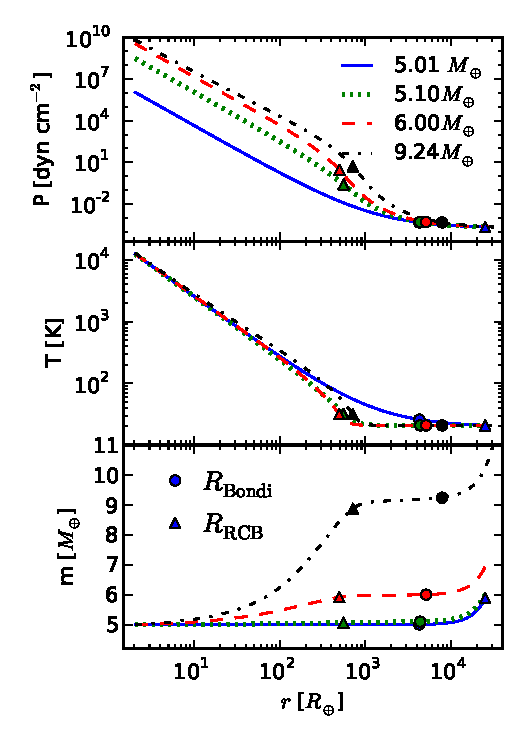
\includegraphics[width=0.5\textwidth]{../../figs/ModelAtmospheres/RadSelfGravPoly/PaperFigs/PTm_profiles_v2_smallM.pdf}
%\vspace{-0.5in}
\caption{Radial profiles of atmospheric pressure, temperature and enclosed mass (including the core) for a $5 M_{\oplus}$ core at $a=60$ AU.   Solid, dotted and dashed lines correspond to solutions with total mass (core and atmosphere) of $5.01 M_{\oplus}$, $5.10 M_{\oplus}$, $6.00 M_{\oplus}$ and $9.24 M_{\oplus}$, respectively.  (See text for a description of evolution to yet higher masses.)   Circles and triangles mark the locations of the Bondi radii and of the radiative-convective boundaries, respectively.  The radial profiles extend from the core to the Hill radius.} 
\label{fig:profiles}
\end{figure}


\subsection{Atmospheric Stucture}
\label{sec:profiles}
Figure \ref{fig:profiles} shows radial profiles at different stages of atmospheric growth.  In these examples, we fix the core mass at $M_{\rm{c}}=5 M_{\oplus}$ and the radial disk location to $a=60$ AU.  The quoted mass values include the core plus atmosphere within the smaller of $\RB$ or $\RH$, which for these cases is $\RB$.  The 9.24 $M_{\oplus}$ solution is the highest mass we can reach in our evolutionary sequence, as we explain further in \S\ref{sec:endoftime}.

Deep in a non-self-gravitating atmosphere, \Eq{eq:deep} shows that $T \propto r^{-1}$ and $P\propto r^{-1/\delad}$.  This behavior is seen in the low mass solutions in \Fig{fig:profiles}.  As explained by \Eq{eq:TPsg}, the higher mass solutions show a flatter profile in $T$ and also in $P \propto T^{1/\delad}$.  In agreement with \Eq{eq:cb2}, the radiative zone remains nearly isothermal -- even in the more massive solutions -- and thus shows a nearly exponential increase in pressure with inverse depth.  

The atmosphere starts out as purely convective and isentropic, as seen in \Fig{fig:profiles} for the 5.01 $M_{\oplus}$ solution which has no radiative zone. Further gas accumulation brings in energy that has to be radiated away, forming a radiative region that quickly deepens. The fast pressure deepening of the radiative region is evident in \Fig{fig:profiles} --- even a low mass atmosphere (i.e. the 5.10 $M_{\oplus}$ solution) has an extended radiative zone. 
 
The higher mass atmosphere solutions have lower entropy, i.e.\ cooling allows the atmosphere to accrete more gas.  This is evident in \Fig{fig:profiles} from the higher internal pressures of the higher mass solutions.  The somewhat higher temperatures in the higher mass solutions do not cause the entropy to increase.

%AY: to say something about starting at disk entropy (not really needed) we should show it better in the figure.  Also unclear if you want to say much more about evolution before figure 2 shows the evolution.
%In the initial stages of its evolution, the atmosphere is purely convective and isentropic, with an entropy equal to that of the disk. In the context of our numerical model, this is the minimum atmosphere mass for which a hydrostatic solution exists. Further gas accumulation brings in energy that has to be radiated away, and an initially thin outer radiative region forms, which becomes thicker as the atmosphere becomes more massive. 

\subsection{Time Evolution}\label{sec:timeev}

\begin{figure}[tb]
\centering
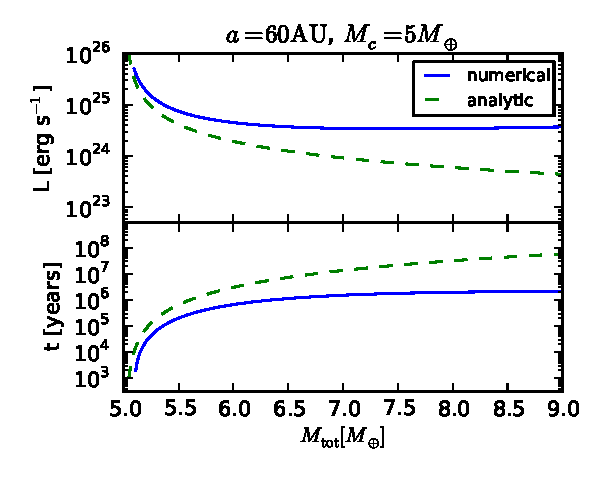
\includegraphics[width=0.5\textwidth]{../../figs/ModelAtmospheres/RadSelfGravPoly/PaperFigs/Lt_profiles_v2.pdf}
%\vspace{-0.5in}
\caption{Evolution of the luminosity and elapsed time during atmospheric growth around a $5 M_{\oplus}$ core at $60$ AU.  The luminosity is initially high, then decreases as the atmosphere grows in mass and the radiative zone becomes optically thicker.  Due to the neglect of self-gravity, the analytic model (\emph{dashed curve}) gives a further drop in luminosity and a longer evolution time.}
\label{fig:Ltplot}
\end{figure}

The cooling model of \S\ref{sec:twolayer} is used to connect solutions of different atmospheric masses into an evolutionary sequence.  \Fig{fig:Ltplot} shows the luminosity evolution and the elapsed time as a function of atmospheric mass for a $5 M_{\oplus}$ core at $60$ AU, i.e.\ the same parameters as in \Fig{fig:profiles}.  During the early stages of atmospheric growth, the luminosity drops sharply.  This behavior is seen in both the full numerical solutions (with solid lines) and the analytic model (with dashed lines).  As seen in \Eq{eq:Lcb}, the increased pressure depth of the RCB increases the optical depth ($\propto \kappa P)$ and decreases the radiative luminosity.

%AY: I don't want to say 5.12 is the lowest mass b/c it's not the adiabat, and I don't see what's gained by saying it's very near the lowest mass.

At later stages of evolution, the numerical model gives a flat luminosity with increasing mass and also time (not shown).  By contrast the analytic model gives a luminosity that continues to drop with increasing mass.  The difference is due to the neglect of self-gravity in the analytic model.  From \Eq{eq:Lcb}, $L\cb \propto M\cb T\cb^4/ (\kappa\cb  P\cb)$.  Thus accounting for the higher enclosed mass gives a somewhat higher luminosity in the self-gravitating model.  However, the main effect is the higher temperature in the self-gravitating models.  The flatter temperature profiles with radius, as described above, explain why the self-gravitating models are hotter.

%The flattening of the luminosity curve is a generic feature of numerical core accretion models

%We find only a brief agreement between the analytic and numerical results. In the early stages, the radiative zone is too shallow and the assumption that $P_{\rm RCB} \gg P_{\rm d}$ used in the analytic model breaks down. 

Before discussing time evolution (both the elapsed time from the bottom panel of \Fig{fig:Ltplot} and the characteristic growth time of the atmosphere), we briefly discuss the effect of decreasing the atmospheric dust abundance on the atmospheric evolution.  In \Fig{fig:LtvsMopacity}, the opacity normalization in \Eq{eq:opacitylaw} is reduced by factors of 10 and 100.  Lower opacities result in higher luminosities and faster evolution, a well-established result \citep{HubBod05} that we confirm for our model.  Atmospheric dust opacities are difficult to robustly predict. Ablation of infalling solids is a dust source, while settling through the radiative zone is a sink.  Grain growth both reduces dust opacities per unit mass and favors settling.  Our scenario of negligible ongoing particle accretion tends to favor low dust opacities.   To be conservative, however, our reference case considers full Solar abundances, but faster evolution is clearly possible. The effect of opacity reduction on the critical core mass is deferred to \S\ref{sec:critical}. 

\begin{figure}[tb]
\centering
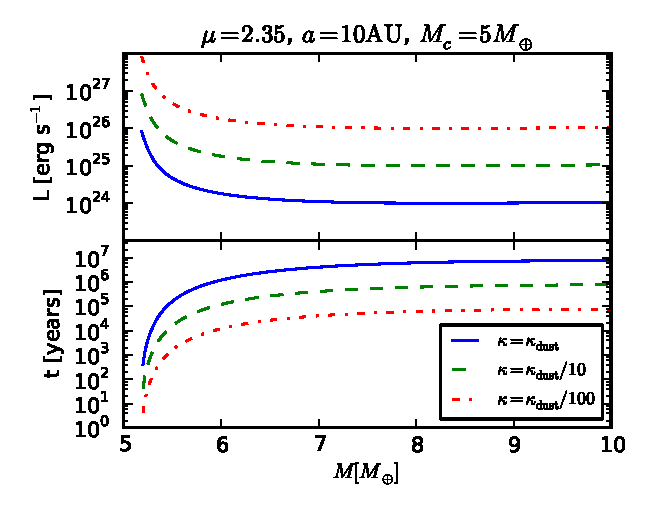
\includegraphics[width=0.5\textwidth]{../../figs/ModelAtmospheres/RadSelfGravPoly/PaperFigs/opacity_effect.pdf}
%\vspace{-0.5in}
\caption{Similar to \Fig{fig:Ltplot}, but showing the effect of reducing the dust abundance by factors of 10 and 100 from standard Solar abundances. The reduced dust opacities give higher luminosities and faster atmospheric growth.}  %The actual magnitude of dust opacities is difficult to robustly predict.}
\label{fig:LtvsMopacity}
\end{figure}

\Fig{fig:growthtime} plots the evolution of the atmospheric growth timescale, $M_{\rm atm}/\dot{M}$,  around a $5 M_{\oplus}$ core at several locations in the disk.  This instantaneous growth time shows clearly that the atmosphere spends the bulk of its time growing though intermediate atmospheric masses, $\sim 1 -3$ $M_\oplus$ in this case.  Growth times are short both early -- when the radiative zone is relatively transparent -- and late -- when self-gravity accelerates growth.  The accelerated growth at higher masses is also evident in \Figs{fig:Ltplot}{fig:LtvsMopacity} (bottom panels) as the flattening of the $t$ vs.\ $M_{\rm atm}$ curve.  

The fact that growth times peak before the crossover mass, when $M_{\rm{atm}} < M_{\rm c}$, is very helpful for understanding atmospheric growth.  The estimated timescale to runaway growth can be well approximated by only considering the time it takes to grow to the crossover mass, or even to a somewhat lower mass.  This insensitivity to the upper mass threshold is characteristic of accelerating growth, and is fortuitious.  We next show how our model assumptions can break down during the later stages of atmospheric growth.

\begin{figure}[tb]
\centering
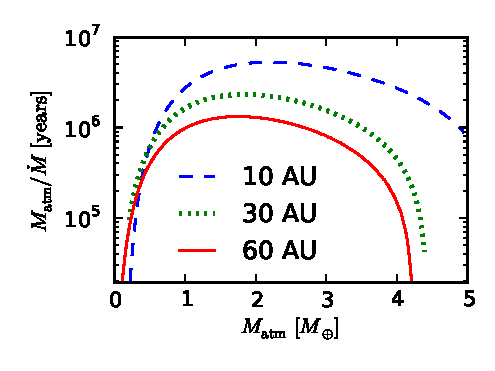
\includegraphics[width=0.5\textwidth]{../../figs/ModelAtmospheres/RadSelfGravPoly/PaperFigs/Mt_profile_temp.pdf}
%\vspace{-0.5in}
\caption{Evolution of the atmospheric growth timescale with mass around a $5 M_{\oplus}$ solid core  located at 10, 30 or 60 AU.  Growth is slowest for $M_{\mathrm{atm}} \sim 1 - 3 M_{\oplus}$, i.e.\ before the crossover mass at $M_{\rm atm} = M\co$.}
\label{fig:growthtime}
\end{figure}

\subsection{Validity of the Two-Layer Cooling Model}
\label{sec:endoftime}

To examine the regimes where our cooling model is valid, we compare the model luminosity to the additional neglected luminosity, $L_{\rm negl}$, that a more detailed model would have generated in the radiative zone.  To compute $L_{\rm negl}$ we compute the entropy difference between successive radiative zone solutions.  We then integrate the energy equation, $\p L / \p m = - T \p S/ \p t$, over the average depth of the radiative zone.\footnote{While useful as a diagnostic, the neglected luminosity cannot reliably correct the global cooling model because where $L_{\rm negl}$ is significant, the structure of the radiative zone would be inaccurate.}

 \Fig{fig:coolingterms} shows that the neglected luminosity is indeed negligible during the early stages of evolution.  However, $L_{\rm negl}$ exceeds the model luminosity, $L$, at high masses, $M_{\rm atm} > 3 M_\oplus$ in this case, meaning that our model is becoming inaccurate.  Nevertheless, our cooling model gives both conservative and reasonably reliable estimates of core accretion timescales.  Our results are conservative -- in the sense of overestimating growth times -- because the neglected luminosity would give more rapid evolution.  Moreover, our results are reasonably accurate because the bulk of growth time is spent at low masses, when $L_{\rm negl}$ is small and safely neglected.
 
The (non-vanishing) individual terms in the global cooling model of \Eq{eq:coolingglobal}, evaluated at the RCB, are also plotted in \Fig{fig:coolingterms}.  At low masses, the change in energy, $- \dot{E}$, makes the dominant contribution to luminosity.  As the mass increases the surface terms become more significant, led by the accretion energy.  However the surface terms are everywhere smaller than $L_{\rm negl}$.  Thus while the surface terms appear to reduce the total luminosity (compared to $-\dot{E}$), $L_{\rm negl}$ can more than compensate, showing again that our model conservatively underestimates cooling.

At yet higher masses than shown in \Fig{fig:coolingterms}, our cooling model breaks down.  Mathematically, the breakdown manifests as negative timesteps when advancing to a higher atmospheric mass.  This unphysical result has no deep significance, as we already know that the neglected luminosity is large enough to give incorrect results.  Sometimes this breakdown occurs even before the crossover mass is reached.  The main practical effect of this behavior is that we halt the evolution where the model breaks down whenever we cannot reach the crossover mass.   Fortunately, the elapsed time to either the crossover mass or the breakdown is well-behaved and, most importantly, dominated by lower atmospheric masses where the model is accurate.  

 
\begin{figure}[tb]
\centering
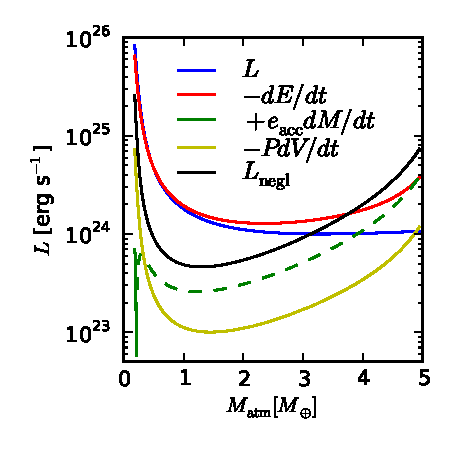
\includegraphics[width=0.5\textwidth]{../../figs/ModelAtmospheres/RadSelfGravPoly/PaperFigs/cooling_a10_Mc5_rcb_paper.pdf}
%\vspace{-0.5in}
%\caption{Luminosity evolution around a $5 M_\oplus$ core at 10 AU.  In addition to the total model luminosity $L$, the contributing terms in the cooling model of \Eq{eq:coolingglobal}; $-\dot{E}$, $e_{\rm M} \dot{M}$ and $-P \p V/ \p t |_M$; are shown.  The $L_{\rm negl}$ curve gives the neglected luminosity that would have been generated in the radiative zone, but is not included in our two-layer cooling model.}
\label{fig:coolingterms}
\end{figure}



\section{Critical Core Mass}
\label{sec:critical}

%AY make sure this AU range comment is incorporated in some form:  We are primarily interested in the outer regions of the disk, so we generate atmosphere models at distances between 5 and 100 AU in our fiducial disk. We emphasize that the location in the disk only affects the temperature and pressure of the nebular gas. As our model applies only when planetesimal accretion occurs too slowly to substantially change the mass of the core, we consider the evolution of an atmosphere around a core of fixed mass.  

\subsection{Disk Temperature and Pressure}
\label{sec:TPeffects}

\section{Neglected Effects}\label{sec:neglected}

\subsection{Hydrodynamic Effects}\label{sec:hydro}
The neglect of hydrodynamical effects in our model is best discussed in terms of the thermal mass, $M_{\rm th}$, and the length scales introduced in \S\ref{sec:scales}.  In the low mass regime, $M\pla < M_{\rm th}/ \sqrt{3}$, where $\RB < \RH$, we assume that hydrostatic balance holds out to the outer boundary at $\RH$.   In this low mass regime, \citet[]{Orm13} calculated the flow patterns driven by stellar tides and disk headwinds.     On scales $\gtrsim \RB$ the flows no longer circulate the planet: they belong to the disk.  Nevertheless, the density structure outside $\RB$ remains spherically symmetric and hydrostatic.  Even if these flows do not destroy hydrostatic balance, they could affect the planet's cooling.  We expect such effects to be weak, as heat losses at greater depths dominate planetary cooling, but more study is needed.

At higher masses, non-hydrostatic effects become more severe.  At $M\pla \gtrsim M_{\rm th}$ planets can open significant gaps \citep{zhu13}.  At yet higher masses accretion instabilities could occur \citep{AylBat12}.  However, in this high mass regime we already know that the spherically symmetric approximation breaks down (see \S\ref{sec:scales}). %, as does our approximate cooling model (\emph{discuss elsewhere and cite}).

Thus by restricting our attention to low masses, neglected hydrodynamic effects should be minor.   Moreover since $M_{\rm th} \propto a^{6/7}$ increases with disk radius, spherical hydrostratic models like ours have a greater range of applicability in the outer regions of disks. 


\subsection{Realistic Opacities}\label{sec:op}
%\emph{some comments on sublimation and radiative windows here (current text rough). upshot is the outer disk is good.}

Real dust opacities exhibit a more complicated behavior that depends on grain composition.  Opacities drop by order unity when ice grains sublimate for $T \gtrsim 150$ K and they drop by orders of magnitude when silicate grains evaporate above $T \gtrsim 1500$ K \citep{semenov03, FerAle05}. Our model assumes that radiative regions only exist in the outer part of the atmosphere. As such, even though protoplanetary atmospheres get significantly hotter than 1500 K, our model depends on opacity only in the upper radiative zones, which are cool enough to remain dusty. For our opacity approximations to be valid, we must restrict our model to the lower temperatures of the outer disk.   

A second radiative zone inside the convection zone, a ``radiative window," is possible, due to the opacity drops caused by the evaporation of ice and metal grains. Our two layer model ignores such complications. Grain growth also impacts the opacity in the outer regions as well as the existence or depth of radiative windows. We explore more realistic opacity laws in  In Piso et al. (2013, in prep.).

% we show that the existence of inner radiative windows does not impact our simplified model significantly, i.e. most of the luminosity is generated in the innermost convective region of the atmosphere and therefore the assumption that luminosity is constant in the radiative layers still holds. 


 \subsection{Equation of State}
 \label{sec:EOS}
 
 In our model we assume an ideal gas law and a polytropic EOS, given by equations (\ref{eq:idealgas}) and (\ref{eq:polyEOS}), respectively. However, non-ideal effects such as partial dissociation and ionization have to be taken into account. One solution is using tabulated equation of state tables for hydrogen and helium mixtures. In Piso et al. (2013, in prep) we use the \citet{saumon95} EOS tables and extend them to lower pressures and temperatures as required by our disk assumptions.



\section{Conclusions} \label{sec:conclusions}

\bibliographystyle{apj}
\bibliography{refs}

\appendix
\section{Derivation of the Global Energy Equation}\label{sec:globalderiv}

To derive  the global energy equation (\ref{eq:coolingglobal}) for an embedded protoplanets, we generalize the analogous calculations in stellar structure theory, e.g.\ in \S4.3 of \citet{kippenhahn90}.  For our problem we add the effects of finite core radius, surface pressure and mass accretion.We start with the local energy equation (\ref{eq:structd}) whose more natural form in Lagrangian (mass) coordinates is $\p L/ \p m = \epsilon - T \p S /\p t$.  Integrating from the core to a higher shell with enclosed mass $M$ gives:
\begin{subeqnarray}
L - L\co &=& \int_{M\co}^M {\p L \over \p m} dm \\
&=& \int_{M\co}^M \left(\epsilon - T {\p S \over \p t} \right)dm \\
&=& \Gamma  - \int_{M\co}^M{\p u \over \p t} dm +  \int_{M\co}^M {P \over \rho^2} {\p \rho \over \p t} dm\slabel{eq:DLc}\, .
\end{subeqnarray} 
with $\Gamma = \int \epsilon dm$ the integral of the direct heating rate and applying the law of thermodynamics in the final step.

The global energy equation is derived by eliminating the partial time derivatives in \Eq{eq:DLc}, which are performed at a fixed mass,
in favor of total time derivatives, denoted with overdots.  %The physical distinction is that total derivatives include mass  accreted through the outer boundary.  
For instance the surface radius, $R$, evolves as  
\begin{equation}\label{eq:Rdot}
 \dot{R} = {\p R \over \p t} + {\dot{M} \over 4 \pi R^2 \rho_M}
\end{equation} 
where $\p R/\p t$ gives the Lagrangian contraction of the ``original" shell, and mass accretion through the upper boundary at rate $\dot{M}$ also changes the shell location.  
%The subscript $M$  denotes quantities at the upper boundary of total mass $M$ (though it is omitted from $M$ and $R$).  
Similarly the volume, $V = (4 \pi/3)r^3$, and pressure at the outer shell evolve as
\begin{subeqnarray}\label{eq:dot}
\dot{V}_M &=&  {\p V_{\rm M} \over \p t} + {\dot{M} \over \rho_{\rm M}}  \\
 \dot{P}_M &=& {\p P_{\rm M} \over \p t} + {\p P_M \over \p m}\dot{M} =  {\p P_{\rm M} \over \p t} - {G M  \over 4 \pi R^4} \dot{M}\, .
\end{subeqnarray} 
This derivation holds the core mass and radius fixed, $\dot{M}\co = \dot{R}\co = 0$.  Therefore the core pressure satisfies
\begin{equation}\label{eq:Pcdot}
 \dot{P}\co = \p P\co / \p t \, .
\end{equation}

The internal energy integral follows simply from  Leibniz's rule as
\begin{equation}\label{eq:udot}
\int_{M\co}^{M(t)}{\p u \over \p t} dm = \dot{U}  -  \dot{M}u_M\, .
\end{equation} 

To make further progress we require the virial theorem:
\begin{equation}
\label{eq:virial}
E_G=-3 \int_{M\co}^M \frac{P}{\rho} dm + 4 \pi (R^3 P_M-R\co^3 P\co)
\end{equation}
which follows from \Eqsss{eq:structb}{eq:structa}{eq:Eg} by integrating hydrostatic balance in Lagrangian coordinates.  As an aside, the integral in equation (\ref{eq:virial}) can be evaluated for a polytropic EOS to give simple expressions for the total energy:
\begin{subeqnarray}
E&=&(1-\zeta)U+4 \pi (R^3 P_M-R\co^3 P\co) \slabel{eq:vira} \\
&=&\frac{\zeta-1}{\zeta}E_G+\frac{4 \pi}{\zeta} (R^3 P_M-R\co^3 P\co) \slabel{eq:virb}
\end{subeqnarray}
where $\zeta \equiv 3(\gamma - 1)$.  We will not make this assumption and will keep the EOS general.

To express the work integral, the final term in \Eq{eq:DLc}, in terms of changes to gravitational energy we first take the
 time derivative of \Eq{eq:virial}:
\begin{eqnarray}\label{eq:EGdot}
\dot{E}_G = 3  \int_{M\co}^M {P \over \rho^2} {\p \rho \over \p t} dm -3 \int_{M\co}^M {\p P\over \p t}{dm \over \rho} 
 -  3{P_M \over \rho_M} \dot{M}+ 3 \dot{P}_M V_M -3 \dot{P}\co V\co  + 3  P_M {\dot{ V}_M} \, . 
\end{eqnarray} 
%where the volumes, $V_M = 4 \pi R^3/3$ and $V\co = 4 \pi R\co^3/3$. 
The first integral in \Eq{eq:EGdot} is the one we want, but the next one must be eliminated.  The time derivative of \Eq{eq:Eg} (times four) gives
\begin{subeqnarray}
 4 \dot{E}_G &=&  -4 {G M \dot{M} \over R} + 4 \int_{M\co}^M {G m \over r^2}{\p r \over \p t} dm\\ 
&=&   -4 {G M \dot{M} \over R} + 4 \pi \int_{M\co}^M r^3{\p \over \p m}{\p P \over \p t} dm \slabel{eq:4EGb} \\
&=&  -4 {G M \dot{M} \over R} -3  \int_{M\co}^M {\p P\over \p t}{dm \over \rho}  + 3 V_M {\p P_M \over \p t} -3 V\co {\p P\co \over \p t} \slabel{eq:4EGc}
\end{subeqnarray} 
where \Eqs{eq:4EGb}{eq:4EGc} use hydrostatic balance  and integration by parts.

%To eliminate the time derivates of pressure, we take the time derivative of the hydrostatic balance equation for $\p^2 P / \p m\p t$ and integrate over $4\pi r^3 dm$ (as in the virial equation derivation) to get
%\begin{equation}\label{eq:dHBdt}
%3 \dot{P}_M V_M -3 \dot{P}\co V\co -3 \int_{M\co}^M {\p P\over \p t}{dm \over \rho}  = 4 \dot{E}_G + 4{G M \over R} \dot{M}  \, .
%\end{equation} 
%Combining \Eqs{eq:EGdot}{eq:dHBdt} gives 
%\begin{eqnarray}\label{eq:rhodot}
%\int_{M\co}^M {P \over \rho^2} {\p \rho \over \p t} dm  &=& - \dot{E}_G - {4 \over 3}{G M\over R} \dot{M} + {P_M \over \rho_M} \dot{M} -  P_M \dot{V}_M  \, , \nonumber \\
%&=&- \dot{E}_G - {4 \over 3}{G M\over R} \dot{M}  -  P_M {\p V_M \over \p t}  \, ,
%\end{eqnarray} 
%where the final step uses \Eq{eq:Rdot}.

Subtracting \Eqs{eq:udot}{eq:4EGc} and rearranging terms with the help of \Eqsss{eq:Rdot}{eq:dot}{eq:Pcdot} gives
\begin{eqnarray}\label{eq:PdVint}
\int_{M\co}^M {P \over \rho^2} {\p \rho \over \p t} dm  &=&  - \dot{E}_G - {G M \dot{M} \over R} - P_M {\p V_M \over \p t} \,  .
\end{eqnarray} 
Combining \Eqsss{eq:DLc}{eq:udot}{eq:PdVint}, we reproduce \Eq{eq:coolingglobal} with the accreted specific energy $e_M \equiv u_M - GM/R$.  

\section{Analytic Cooling Model Details}\label{sec:analytic}
TODO (academic): Figure out if theta < 1 is actually required? Should be but need to check

\end{document}



